\documentclass[12pt]{article}
%\usepackage{xr} % % % UNCOMMENT BELOW IF YOU WANT TO CROSS REF WITH PAPER
%\externaldocument{rstar_v4_appendix}
\usepackage{amssymb}
\usepackage{amsfonts}
%\usepackage[dvips]{color}
\usepackage{graphicx}
\usepackage{amsmath}
\usepackage{amsthm}
\usepackage{rotating}
\usepackage{float}              % for specifying [H] option in figures
\usepackage{changepage}         % For adjustwidth to tables
\usepackage{pgffor}             % for for loops (\foreach)
\usepackage{subcaption}         % for sub-figures
\usepackage{standalone}         % to load in the table .tex file using \input w/o removing preamble
\usepackage{algorithm}              % For algorithm
\usepackage[noend]{algpseudocode}   % For algorithm
\usepackage{xcolor}
\usepackage[pdftex,pdfstartview=FitH,bookmarksopen,colorlinks,citecolor=black,    urlcolor=blue,filecolor=black,linkcolor=blue,naturalnames]{hyperref}

\usepackage{epsfig}
\usepackage{natbib}
\usepackage{fancyhdr}

\usepackage{titlesec}

\titleclass{\subsubsubsection}{straight}[\subsection]
\newcounter{subsubsubsection}[subsubsection]
\renewcommand\thesubsubsubsection{\thesubsubsection.\arabic{subsubsubsection}}
\titleformat{\subsubsubsection}
    {\normalfont\normalsize\bfseries}{\thesubsubsubsection}{1em}{}
\titlespacing*{\subsubsubsection}
{0pt}{3.25ex plus 1ex minus .2ex}{1.5ex plus .2ex}

\bibliographystyle{aer}

\pagestyle{myheadings}
%\markright{Del Negro, Schorfheide -- DSGE Model Based Forecasting: \today}
\parindent20pt
\parskip1ex plus1.5ex minus0.2ex
\setcounter{secnumdepth}{5}
\setcounter{tocdepth}{2}

\voffset0cm
\topmargin0cm

%Paper Style
%twoside
\oddsidemargin0cm
\evensidemargin0cm
\textheight8.6in
\textwidth6.5in
\renewcommand{\baselinestretch}{1.3}

%Draft STYLE
%\oddsidemargin-0.5cm
%\evensidemargin0cm
%\textheight8.6in
%\textwidth5.5in
%\renewcommand{\baselinestretch}{1.5}

\newcommand{\fra}[2]{\frac{\displaystyle #1}{\displaystyle #2}}
\newcommand{\bc}{\begin{center}}
	\newcommand{\ec}{\end{center}}
\newcommand{\be}{\begin{equation}}
\newcommand{\ee}{\end{equation}}
\newcommand{\bea}{\begin{eqnarray}}
\newcommand{\eea}{\end{eqnarray}}
\newcommand{\bean}{\begin{eqnarray*}}
	\newcommand{\eean}{\end{eqnarray*}}
\def\ba{\begin{array}}
\def\ea{\end{array}}
\newcommand{\refline}{\raisebox{1ex}{\underline{\hspace{2cm}} \quad}}


\theoremstyle{definition}
\newtheorem{theorem}{Theorem}
\newtheorem{definition}{Definition}
\newtheorem{lemma}{Lemma}
\newtheorem{corollary}{Corollary}
\newtheorem{proposition}{Proposition}
\newtheorem{assumption}{Assumption}
\newtheorem{algo}{Algorithm}

\newcounter{pkt}
\newenvironment{tlist}%
{\begin{list}{(\roman{pkt})}{\usecounter{pkt}\parskip0ex\parsep0ex\itemsep0ex\topsep0ex}}%
	{\end{list}}


\def\EE{\mathord{I\kern-.35em E}}
\def\PP{\mathord{I\kern-.3em P}}
\def\QQ{\mathord{Q\kern-5pt\hbox{\raise1.1pt\hbox{\vrule height5pt}}\kern5pt}}
\def\RR{\mathord{I\kern-.3em R}}

\def\I{{\cal I}}
\def\p{{\cal P}}
\def\E{{\cal E}}
\def\F{{\cal F}}
\def\S{{\cal S}}
\def\Q{{\cal Q}}
\def\L{{\cal L}}
\def\M{{\cal M}}
\def\N{{\cal N}}
\def\T{{\cal T}}
\def\w{w^r}


\usepackage{xcolor}
\DefineNamedColor{named}{myblue}{rgb}{.2,.5,1} %%light blue
\DefineNamedColor{named}{mygreen}{rgb}{.1 .5 .2}
\DefineNamedColor{named}{mypurple}{rgb}{.75 .2 .75}
\newcommand{\cb}{\color{myblue}} % Marco
\newcommand{\cg}{\color{mygreen}} % Abhi
\newcommand{\cp}{\color{mypurple}} % Pearl

\usepackage{booktabs}
\usepackage[justification=centering]{caption}
\usepackage[margin=1in]{geometry}
\usepackage{longtable}
\usepackage{cellspace} % For adding space between parameter group separators ("Policy", etc.)
\setlength\cellspacetoplimit{7pt}
\setlength\cellspacebottomlimit{7pt}

\newcounter{saveeqn}%

%% track changes
%% use the following line if you want changes to show
%\usepackage[]{trackchanges2}
%\renewcommand{\initialsOne}{MDN}

\usepackage{float} %\restylefloat{table}

\everymath{\displaystyle}
%\setlength{\parindent}{0mm}

% Set base directories for bibliography and figures
\newcommand\plotroot{../figures_for_paper}

\begin{document}
	%DSGE Model Estimation and Forecasting using Sequential Monte Carlo Methods

\title{\bf \vspace*{-2cm} Figures/Tables Replication}
\author{Michael Cai, Marco Del Negro, Edward Herbst, \\ Ethan Matlin, Rebecca Sarfati, Frank Schorfheide\thanks{
Correspondence:  Michael Cai \texttt{michaelcai@u.northwestern.edu},
Marco Del Negro \texttt{marco.delnegro@ny.frb.org},
Edward Herbst \texttt{edward.p.herbst@frb.gov},
Ethan Matlin \texttt{ethan.matlin@ny.frb.org},
Rebecca Sarfati \texttt{rebecca.sarfati@ny.frb.org},
Frank Schorfheide \texttt{schorf@ssc.upenn.edu}.
We thank participants at various conferences and seminars for helpful comments. Schorfheide acknowledges financial support from the National Science Foundation under Grant SES 1851634.
The views expressed in this paper are those of the authors and do not necessarily reflect the position of the Federal Reserve Bank of New York, the Federal Reserve Board or the Federal Reserve System.\setlength{\baselineskip}{4mm} } \\
{\small {\em Northwestern University, FRB New York, Federal Reserve Board, }} \\
{\small {\em FRB New York, University of Pennsylvania}}}

\date{\today}
\maketitle

\thispagestyle{empty}

%\newpage

\section{SMC Estimation at Work}\label{sec:estimation}
\begin{table}[H]
    \caption{AS Model: Fixed and Adaptive Tempering Schedules}
    \label{tab:as.smcsummary}
    \begin{center}
        \begin{tabular} {lrrrrrr} 
 \hline \hline 
&Fixed&$\alpha = $0.90&$\alpha = $0.95&$\alpha = $0.97&$\alpha = $0.98\\ 
 \hline 
Mean log(MDD)&-1032.60&-1034.21&-1032.48&-1032.07&-1031.92\\ 
StdD log(MDD)&0.76&1.48&0.61&0.32&0.22\\ 
Schedule Length&200.00&112.17&218.80&350.06&505.46\\ 
Resamples&14.63&15.37&15.03&14.99&14.00\\ 
Runtime [Min]&1.29&0.88&1.53&2.21&3.13\\ 
\hline 
\end{tabular}
    \end{center}
    %\hspace*{-1cm}
    {\footnotesize {\em Notes:} Results are based on $N_{run} = 400$ runs of the SMC algorithm. We report averages across runs for the runtime, schedule length, and number of resampling steps.}\setlength{\baselineskip}{4mm}
\end{table}

\begin{table}[H]
    \caption{SW Model: Fixed and Adaptive Tempering Schedules}
    \label{tab:sw.smcsummary}
    \begin{center}
        \begin{tabular} {lrrrrrr} 
 \hline \hline 
&Fixed&$\alpha = $0.90&$\alpha = $0.95&$\alpha = $0.97&$\alpha = $0.98\\ 
 \hline 
Mean log(MDD)&-1178.43&-1186.23&-1180.04&-1178.31&-1177.72\\ 
StdD log(MDD)&1.34&3.07&1.53&1.03&1.01\\ 
Schedule Length&500.00&200.53&389.75&618.53&887.42\\ 
Resamples&26.75&28.09&27.25&26.33&25.09\\ 
Runtime [Min]&80.23&31.36&61.29&97.79&139.99\\ 
\hline 
\end{tabular}
    \end{center}
    %\hspace*{-1cm}
    {\footnotesize {\em Notes:} Results are based on $N_{run} = 200$ runs of the SMC algorithm. We report averages across runs for the runtime, schedule length, and number of resampling steps.}\setlength{\baselineskip}{4mm}
\end{table}

\begin{figure}[H]
    \caption{Trade-Off Between Runtime and Accuracy}
    \label{fig:smc_time_v_accuracy}
    \begin{center}
        \begin{tabular}{cc}
            AS Model & SW Model \\
            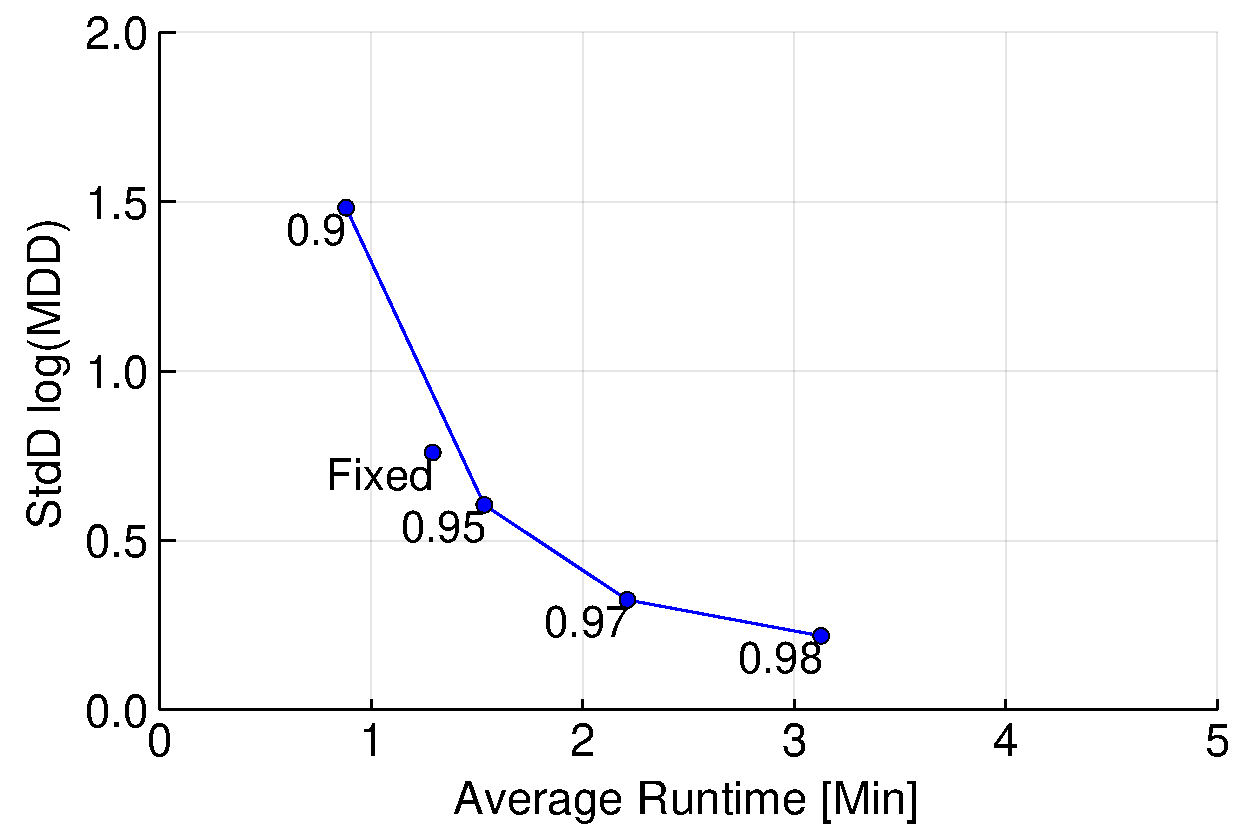
\includegraphics[width = 0.47\textwidth]{\plotroot/estimation/adaptive/as/figure_1_as_mh1_StdVsTime.pdf} &
            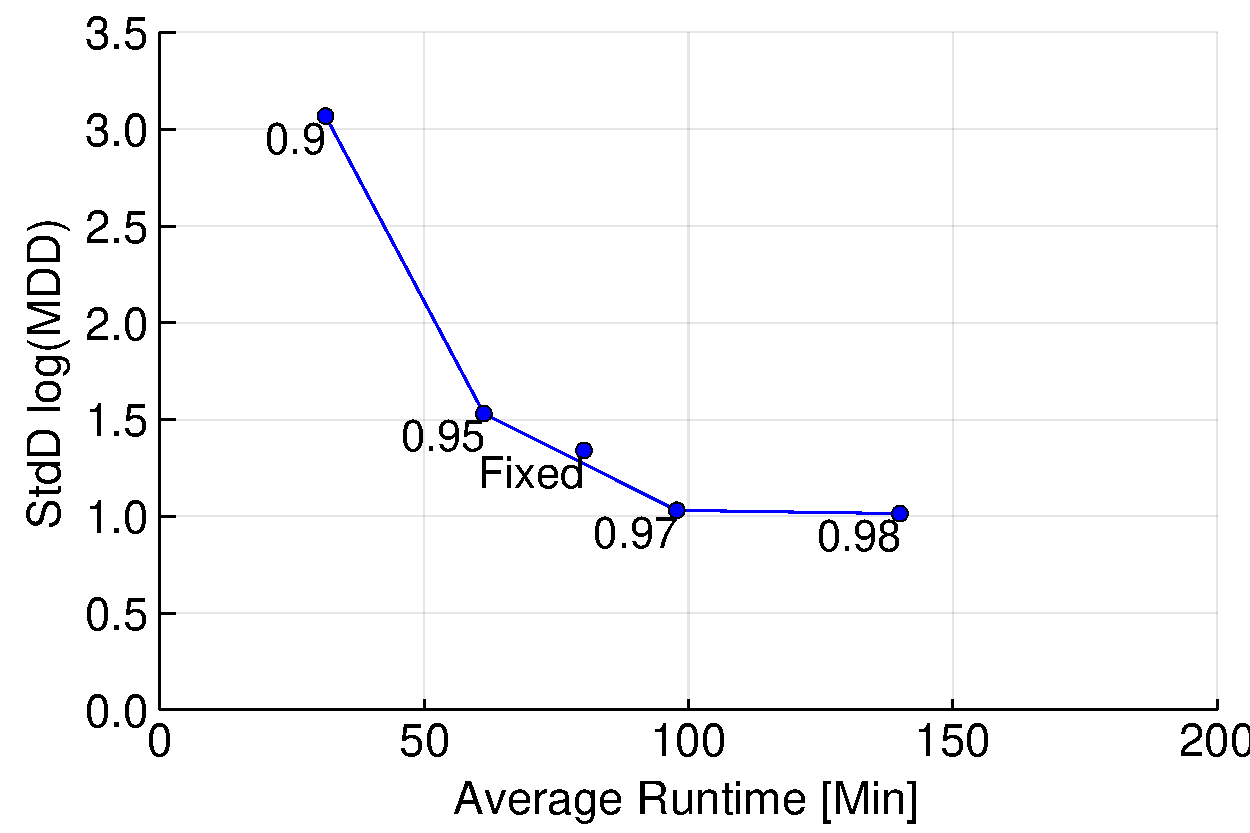
\includegraphics[width = 0.47\textwidth]{\plotroot/estimation/adaptive/sw/figure_1_sw_mh1_StdVsTime.pdf}
        \end{tabular}
    \end{center}
    {\footnotesize {\em Notes:} AS results are based on $N_{run} = 400$ and SW results are based on $N_{run} = 200$ runs of the SMC algorithm.}\setlength{\baselineskip}{4mm}
\end{figure}

\begin{figure}[H]
    \caption{Tempering Schedules}
    \label{fig:smc_tempering}
    \begin{center}
        \begin{tabular}{cc}
        AS Model & SW Model \\
        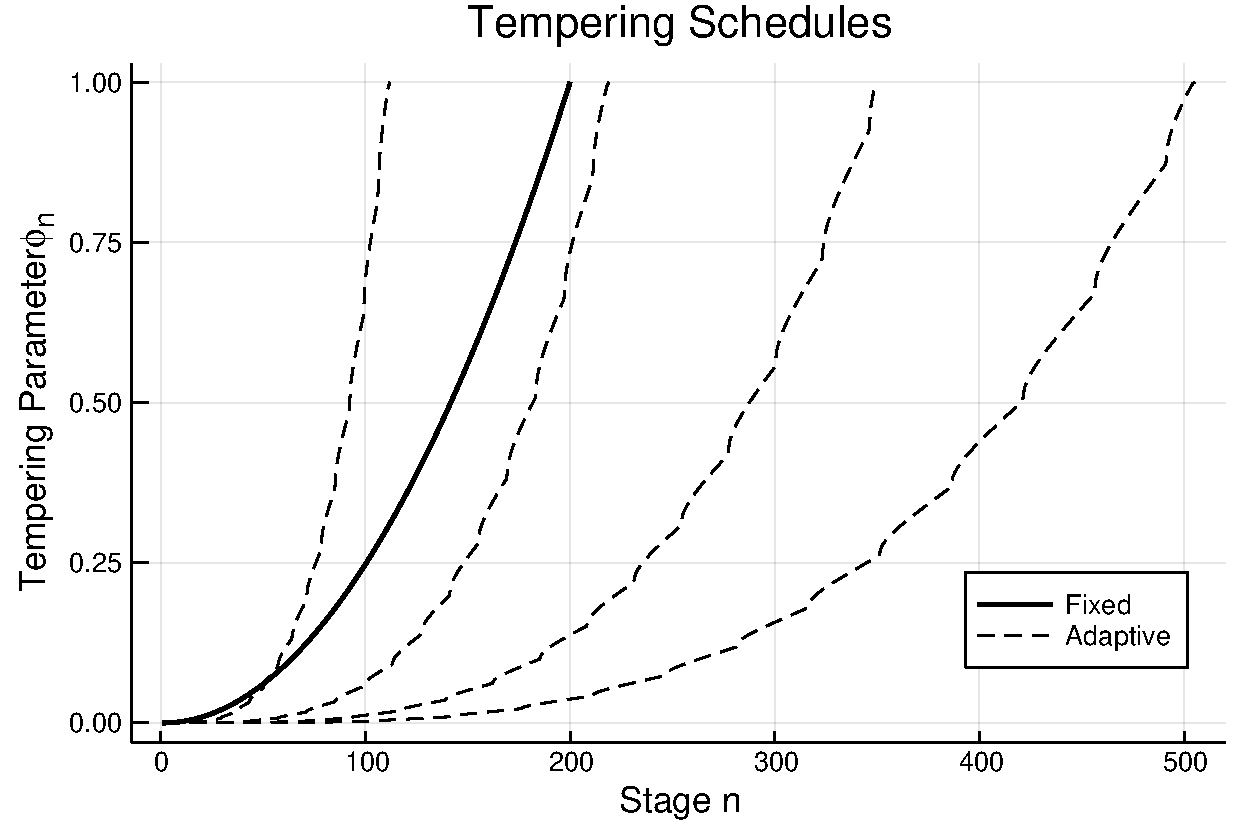
\includegraphics[width=0.47\textwidth]{\plotroot/estimation/adaptive/as/figure_2_tempering_scheds_as_mh1.pdf} &
        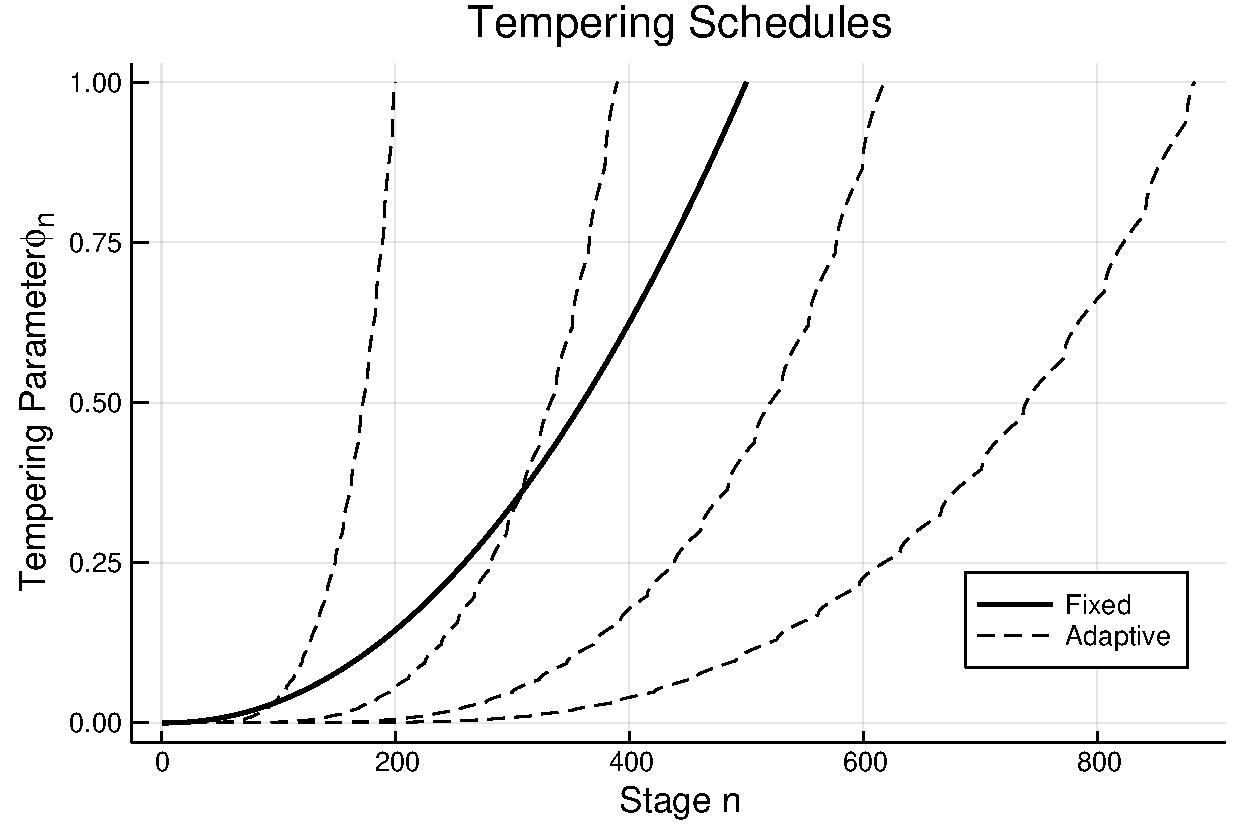
\includegraphics[width=0.47\textwidth]{\plotroot/estimation/adaptive/sw/figure_2_tempering_scheds_sw_mh1.pdf}
        \end{tabular}
    \end{center}
    {\footnotesize {\em Notes:} The figure depicts (pointwise) median $\phi_n$ values across $N_{run} = 200$ for AS and $N_{run} = 100$ for SW. The solid lines represent the fixed schedule, parameterized accord\
ing to Table~\ref{tab:smc.config}. The dashed lines represent a range of adaptive schedules: $\alpha = 0.9, 0.95, 0.97, 0.98$.
}\setlength{\baselineskip}{4mm}
\end{figure}

\begin{figure}[H]
    \caption{Trade-Off Between Runtime and Accuracy -- Multiple Metropolis-Hastings Steps}
    \label{fig:smc_time_v_accuracy_mh}
    \begin{center}
        \begin{tabular}{cc}
        An-Schorfheide & Smets-Wouters \\
        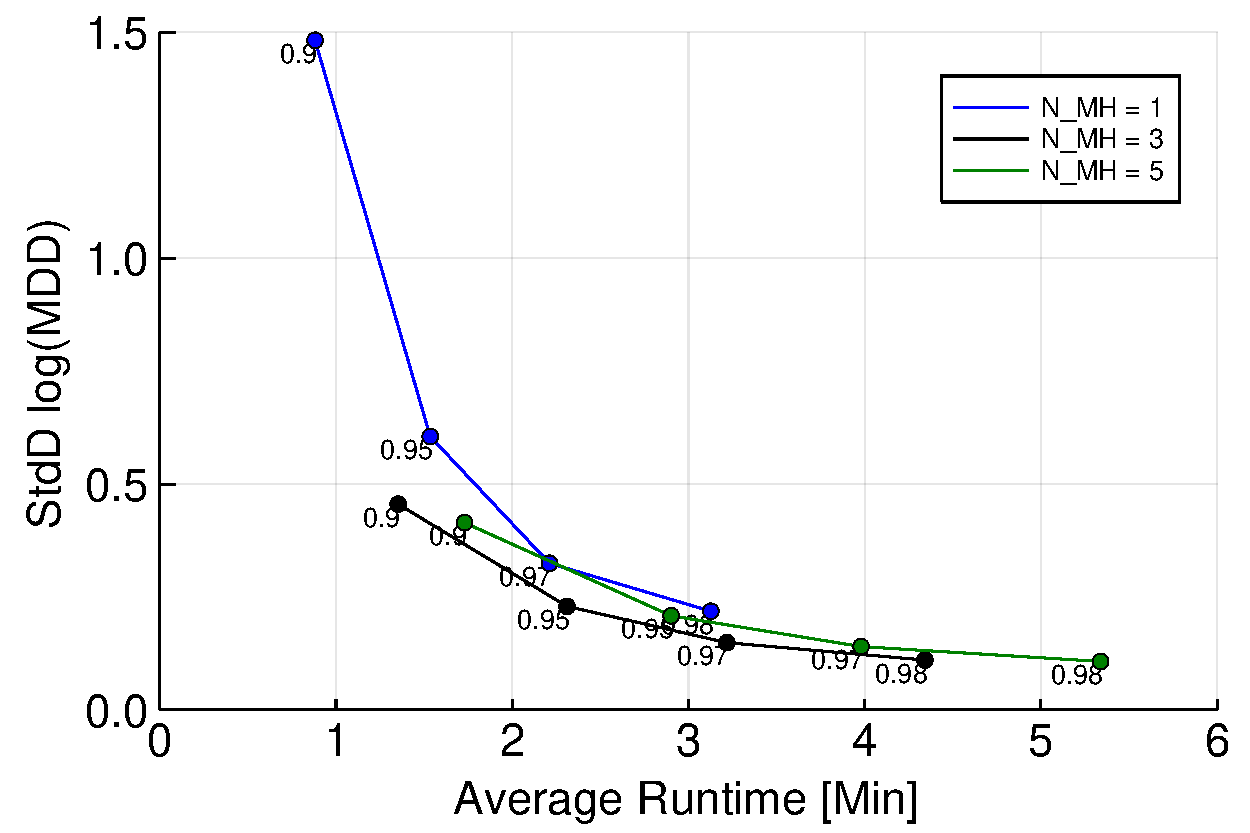
\includegraphics[width = 0.5\textwidth]{\plotroot/estimation/adaptive/as/figure_1_as_mh135_StdVsTime.pdf} &
        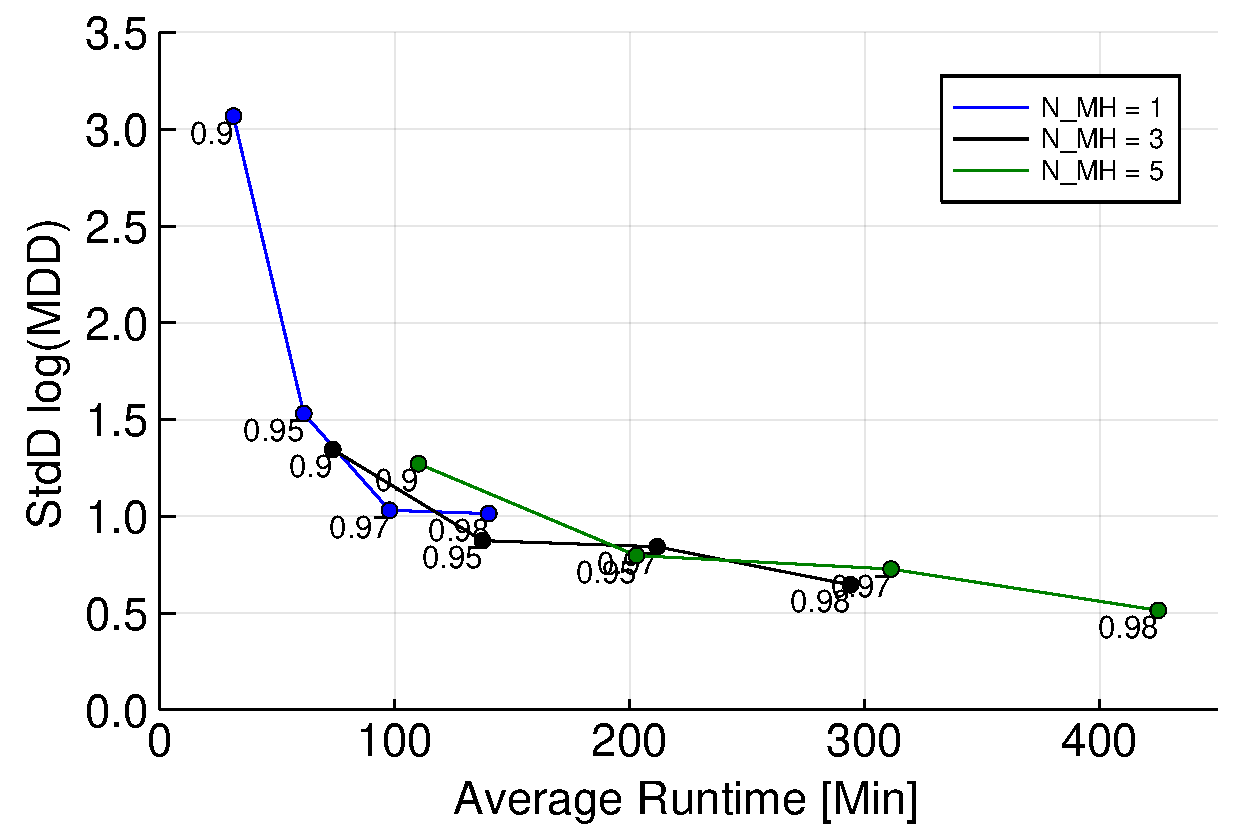
\includegraphics[width = 0.5\textwidth]{\plotroot/estimation/adaptive/sw/figure_1_sw_mh135_StdVsTime.pdf}
        \end{tabular}
    \end{center}
    {\footnotesize {\em Notes:} An-Schorfheide results are based on $N_{run} = 400$ and Smets-Wouters results are based on $N_{run} = 200$ runs of the SMC algorithm.}\setlength{\baselineskip}{4mm}
\end{figure}

\begin{table}[H]
    \caption{AS Model: Generalized Tempering}
    \label{tab:as.smc.full.vs.datatempering}
    \begin{center}
        \begin{tabular} {lrrrrr} 
 \hline \hline 
&$\alpha = $0.90&$\alpha = $0.95&$\alpha = $0.97&$\alpha = $0.98\\ 
 \hline 
Mean log(MDD)&-1033.95&-1032.54&-1032.06&-1031.93\\ 
StdD log(MDD)&1.37&0.61&0.32&0.24\\ 
Schedule Length&24.33&47.12&75.74&106.50\\ 
Runtime [Min]&0.25&0.48&0.69&0.98\\ 
\hline 
\end{tabular}
    \end{center}
    %\hspace*{-1cm}
    {\footnotesize {\em Notes:} Results are based on $N_{run} = 400$ runs of the SMC algorithm, starting from particles that represent $p(\theta|Y_{1:T_1})$. We report averages across runs for the runtime, sche\
dule length, and number of resampling steps.}\setlength{\baselineskip}{4mm}
\end{table}

\begin{table}[H]
    \caption{SW Model: Generalized Tempering}
    \label{tab:sw.smc.full.vs.datatempering}
    \begin{center}
        \begin{tabular} {lrrrrr} 
 \hline \hline 
&$\alpha = $0.90&$\alpha = $0.95&$\alpha = $0.97&$\alpha = $0.98\\ 
 \hline 
Mean log(MDD)&-1188.93&-1182.08&-1180.05&-1178.90\\ 
StdD log(MDD)&3.10&1.83&1.11&1.06\\ 
Schedule Length&56.60&115.73&194.01&290.74\\ 
Runtime [Min]&16.32&33.64&56.79&85.01\\ 
\hline 
\end{tabular}
    \end{center}
    %\hspace*{-1cm}
    {\footnotesize {\em Notes:} Results are based on $N_{run} = 200$ runs of the SMC algorithm, starting from particles that represent $p(\theta|Y_{1:T_1})$. We report averages across runs for the runtime, sche\
dule length, and number of resampling steps.}\setlength{\baselineskip}{4mm}
\end{table}


\begin{figure}[H]
    \caption{Trade-Off Between Runtime and Accuracy}
    \label{fig:smc_time_v_accuracy2}
    \begin{center}
        \begin{tabular}{cc}
            AS Model & SW Model \\
            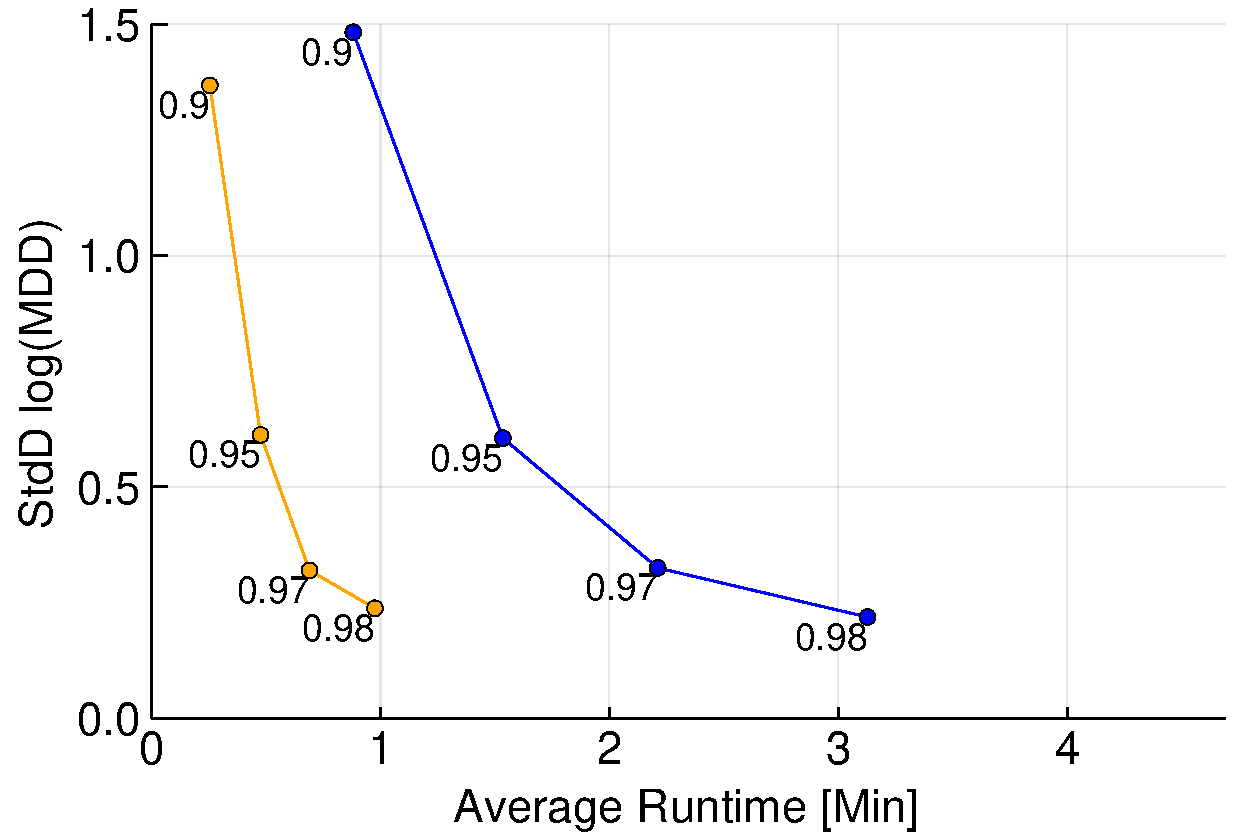
\includegraphics[width = 0.47\textwidth]{\plotroot/estimation/time_temper/as/figure_3_as_mh1_StdVsTime.pdf} &
            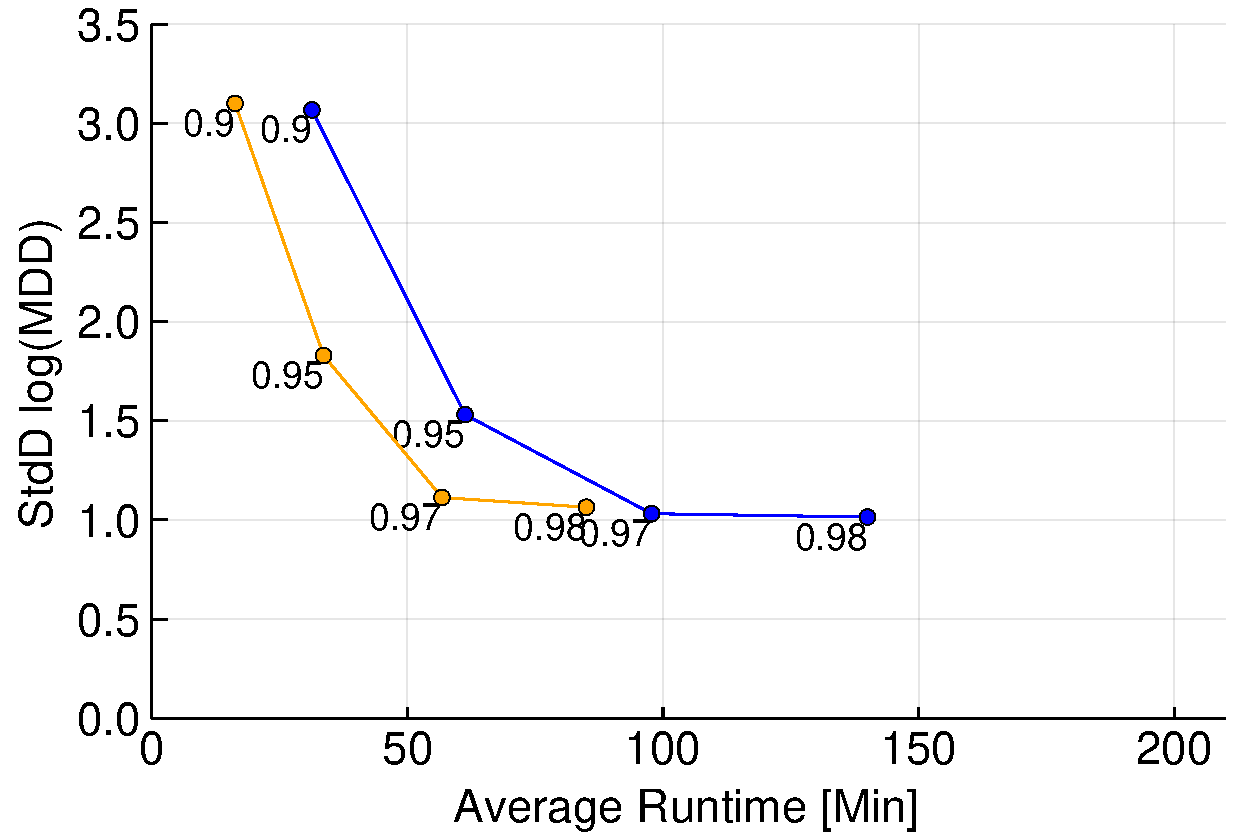
\includegraphics[width = 0.47\textwidth]{\plotroot/estimation/time_temper/sw/figure_3_sw_mh1_StdVsTime.pdf}
        \end{tabular}
    \end{center}
    {\footnotesize {\em Notes:} AS results are based on $N_{run} = 400$ and SW results are based on $N_{run} = 200$ runs of the SMC algorithm. Yellow squares correspond to generalized tempering and blue circles\
 correspond to full sample estimation.
    }\setlength{\baselineskip}{4mm}
\end{figure}

\begin{figure}[H]
    \caption{AS Model: Log MDD Increments $\log(p(y_{T_{s-1}+1:T_s}|y_{1:T_{s-1}}))$}
    \label{fig:smc_time_v_accuracy3}
    \begin{center}
        \begin{tabular}{cc}
            Mean log(MDD) & StdD log(MDD) \\
            \includegraphics[width = 0.45\textwidth]{\plotroot/estimation/time_temper/as/an_schorfheide_exercise/means_over_time_98.pdf} &
            \includegraphics[width = 0.45\textwidth]{\plotroot/estimation/time_temper/as/an_schorfheide_exercise/stds_over_time_98.pdf}
        \end{tabular}
    \end{center}
    {\footnotesize {\em Notes:} Results are based on $N_{run} = 200$ runs of the SMC algorithm with $\alpha=0.95$.}\setlength{\baselineskip}{4mm}
\end{figure}

\begin{figure}[H]
    \caption{AS Model: Evolution of Posterior Means and Coverage Bands}
    \label{fig:smc_posteriorsequence}
    \begin{center}
        \begin{tabular}{cc}
            $\tau$ & $\sigma_R$ \\
            \includegraphics[width = 0.45\textwidth]{\plotroot/estimation/time_temper/as/an_schorfheide_exercise/tau_mean_and_coverage_bands_98.pdf} &
            \includegraphics[width = 0.45\textwidth]{\plotroot/estimation/time_temper/as/an_schorfheide_exercise/sigma_R_mean_and_coverage_bands_98.pdf}
        \end{tabular}
    \end{center}
    {\footnotesize {\em Notes:} Sequence of posterior means (red line) and 90\% coverage bands black lines. The dashed line indicates the temporal average of the posterior means. We use $\alpha = 0.95$ for the \
SMC algorithm.}\setlength{\baselineskip}{4mm}
\end{figure}

\begin{figure}[H]
    \caption{SW Model: Posterior Contours for Selected Parameter Pairs}
    \label{fig:smc.multimodal}
    \begin{center}
        \begin{tabular}{cc}
            Standard Prior & Diffuse Prior \\
            \multicolumn{2}{c}{$\iota_p \text{ and } \rho_{\lambda_f}$}\\
            \includegraphics[height = .2\textheight]{\plotroot/estimation/standard_vs_diffuse/sw/ss1/kdensity_vint=920110_param1=iota_p_param2=rho_{lambda_f}.pdf} &
            \includegraphics[height = .2\textheight]{\plotroot/estimation/standard_vs_diffuse/sw/ss6/kdensity_vint=920110_param1=iota_p_param2=rho_{lambda_f}.pdf} \\
            \multicolumn{2}{c}{$\iota_p \text{ and } \eta_{gz}$}\\
            \includegraphics[height = .2\textheight]{\plotroot/estimation/standard_vs_diffuse/sw/ss1/kdensity_vint=920110_param1=iota_p_param2=eta_{gz}.pdf} &
            \includegraphics[height = .2\textheight]{\plotroot/estimation/standard_vs_diffuse/sw/ss6/kdensity_vint=920110_param1=iota_p_param2=eta_{gz}.pdf} \\
            \multicolumn{2}{c}{$h \text{ and } \rho_{\lambda_f}$}\\
            \includegraphics[height = .2\textheight]{\plotroot/estimation/standard_vs_diffuse/sw/ss1/kdensity_vint=920110_param1=h_param2=rho_{lambda_f}.pdf} &
            \includegraphics[height = .2\textheight]{\plotroot/estimation/standard_vs_diffuse/sw/ss6/kdensity_vint=920110_param1=h_param2=rho_{lambda_f}.pdf}
        \end{tabular}
    \end{center}
    {\footnotesize {\em Notes:} Estimation sample is 1960:Q1 to 1991:Q3. We use $\alpha=0.98$ for the SMC algorithm. Plots show a two-dimensional visualization of the full-dimension joint posterior.}\setlength{\
\baselineskip}{4mm}
\end{figure}

\section{Predictive Density Evaluations}

\subsection{Log Predictive Density Scores with Standard Prior}
\label{subsec:forecasting_standardprior}
\begin{figure}[h!]
    \caption{Average Log Predictive Scores for SW vs SWFF}
    \label{fig:avgpreddens_sw_vs_swff_whole_sample}
      \vspace*{-0.75cm}
  \begin{center}
        \begin{tabular}{@{\hspace*{-.4cm}}ccc}
                    GDP & GDP Deflator & GDP and GDP Deflator \\[-.5ex]
            \multicolumn{3}{c}{Conditioning on Nowcasts and FFR Expectations} \\[-.5ex]
            \includegraphics[height=1.5in,width=.32\textwidth,angle=0,clip, trim=.1cm .1cm .1cm .1cm]{\plotroot/forecasting/predictive_densities/standard_prior/pred_densities_gdp/SWvm904/time_averaged_sw_vs_swff_both_T0=1991-12-31_T=2016-12-31.pdf} &
            \includegraphics[height=1.5in,width=.32\textwidth,angle=0,clip, trim=.1cm .1cm .1cm .1cm]{\plotroot/forecasting/predictive_densities/standard_prior/pred_densities_def/SWvm904/time_averaged_sw_vs_swff_both_T0=1991-12-31_T=2016-12-31.pdf} &
            \includegraphics[height=1.5in,width=.32\textwidth,angle=0,clip, trim=.1cm .1cm .1cm .1cm]{\plotroot/forecasting/predictive_densities/standard_prior/pred_densities_both/SWvm904/time_averaged_sw_vs_swff_both_T0=1991-12-31_T=2016-12-31.pdf} \\[-.5ex]
            \multicolumn{3}{c}{Conditioning on Nowcasts} \\[-.5ex]
            \includegraphics[height=1.5in,width=.32\textwidth,angle=0,clip, trim=.1cm .1cm .1cm .1cm]{\plotroot/forecasting/predictive_densities/standard_prior/pred_densities_gdp/SWvm904/time_averaged_sw_vs_swff_nowcast_T0=1991-12-31_T=2016-12-31.pdf} &
            \includegraphics[height=1.5in,width=.32\textwidth,angle=0,clip, trim=.1cm .1cm .1cm .1cm]{\plotroot/forecasting/predictive_densities/standard_prior/pred_densities_def/SWvm904/time_averaged_sw_vs_swff_nowcast_T0=1991-12-31_T=2016-12-31.pdf} &
            \includegraphics[height=1.5in,width=.32\textwidth,angle=0,clip, trim=.1cm .1cm .1cm .1cm]{\plotroot/forecasting/predictive_densities/standard_prior/pred_densities_both/SWvm904/time_averaged_sw_vs_swff_nowcast_T0=1991-12-31_T=2016-12-31.pdf} \\[-.5ex]
            \multicolumn{3}{c}{Conditioning on FFR Expectations} \\[-.5ex]
            \includegraphics[height=1.5in,width=.32\textwidth,angle=0,clip, trim=.1cm .1cm .1cm .1cm]{\plotroot/forecasting/predictive_densities/standard_prior/pred_densities_gdp/SWvm904/time_averaged_sw_vs_swff_bluechip_T0=1991-12-31_T=2016-12-31.pdf} &
            \includegraphics[height=1.5in,width=.32\textwidth,angle=0,clip, trim=.1cm .1cm .1cm .1cm]{\plotroot/forecasting/predictive_densities/standard_prior/pred_densities_def/SWvm904/time_averaged_sw_vs_swff_bluechip_T0=1991-12-31_T=2016-12-31.pdf} &
            \includegraphics[height=1.5in,width=.32\textwidth,angle=0,clip, trim=.1cm .1cm .1cm .1cm]{\plotroot/forecasting/predictive_densities/standard_prior/pred_densities_both/SWvm904/time_averaged_sw_vs_swff_bluechip_T0=1991-12-31_T=2016-12-31.pdf} \\[-.5ex]
            \multicolumn{3}{c}{Conditioning on Neither} \\[-.5ex]
            \includegraphics[height=1.5in,width=.32\textwidth,angle=0,clip, trim=.1cm .1cm .1cm .1cm]{\plotroot/forecasting/predictive_densities/standard_prior/pred_densities_gdp/SWvm904/time_averaged_sw_vs_swff_neither_T0=1991-12-31_T=2016-12-31.pdf} &
            \includegraphics[height=1.5in,width=.32\textwidth,angle=0,clip, trim=.1cm .1cm .1cm .1cm]{\plotroot/forecasting/predictive_densities/standard_prior/pred_densities_def/SWvm904/time_averaged_sw_vs_swff_neither_T0=1991-12-31_T=2016-12-31.pdf} &
            \includegraphics[height=1.5in,width=.32\textwidth,angle=0,clip, trim=.1cm .1cm .1cm .1cm]{\plotroot/forecasting/predictive_densities/standard_prior/pred_densities_both/SWvm904/time_averaged_sw_vs_swff_neither_T0=1991-12-31_T=2016-12-31.pdf} \\[-.5ex]
        \end{tabular}
    \end{center}
    \begin{minipage}{\textwidth}
        \vspace{-.5cm}
        \scriptsize
        \setlength{\baselineskip}{2mm}
        \emph{Note}: These panels compare the log predictive densities from the SW DSGE Model (blue diamonds) with the SWFF DSGE model (red diamonds) averaged over two, four, six, and eight quarter horizons for output growth and inflation individually, and for both together. Forecast origins from January 1992 to January 2017 only are included in these calculations.
    \end{minipage}
\end{figure}

\begin{figure}[h!]
    \caption{Log Predictive Scores for GDP Growth Over Time --- SW vs SWFF}
    \label{fig:GDPpredictive_densities_over_time}
    \vspace*{-0.75cm}
    \begin{center}
        \begin{tabular}{@{\hspace*{-.4cm}}cc}
            Horizon = 2 & Horizon = 8 \\[-.5ex]
            \multicolumn{2}{c}{Conditioning on Nowcasts and FFR Expectations} \\[-.5ex]
            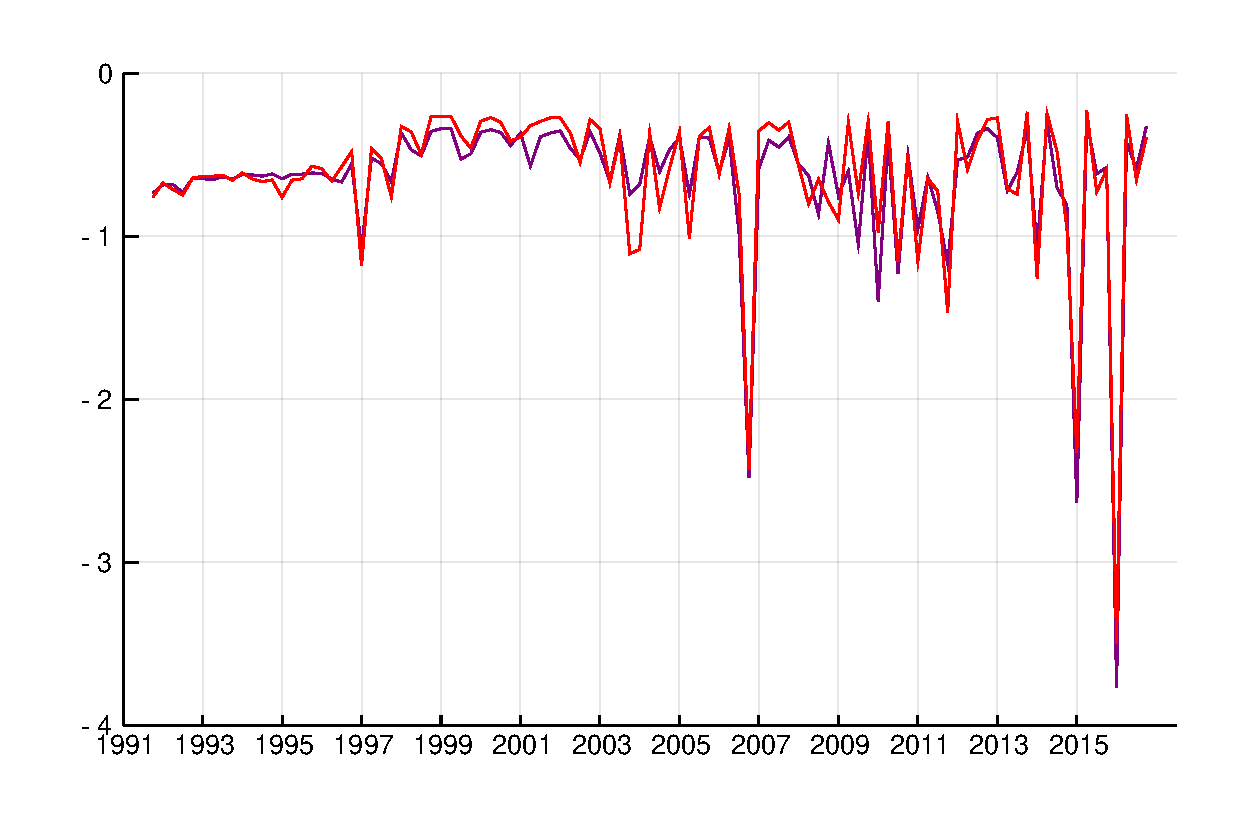
\includegraphics[height=1.5in,width=.45\textwidth,angle=0,clip, trim=.1cm .1cm .1cm .1cm]{\plotroot/forecasting/predictive_densities/standard_prior/pred_densities_gdp/SWvm904/grouped_mean_pred_dens_both_hor=2_T0=1991-12-31_T=2016-12-31.pdf} &
            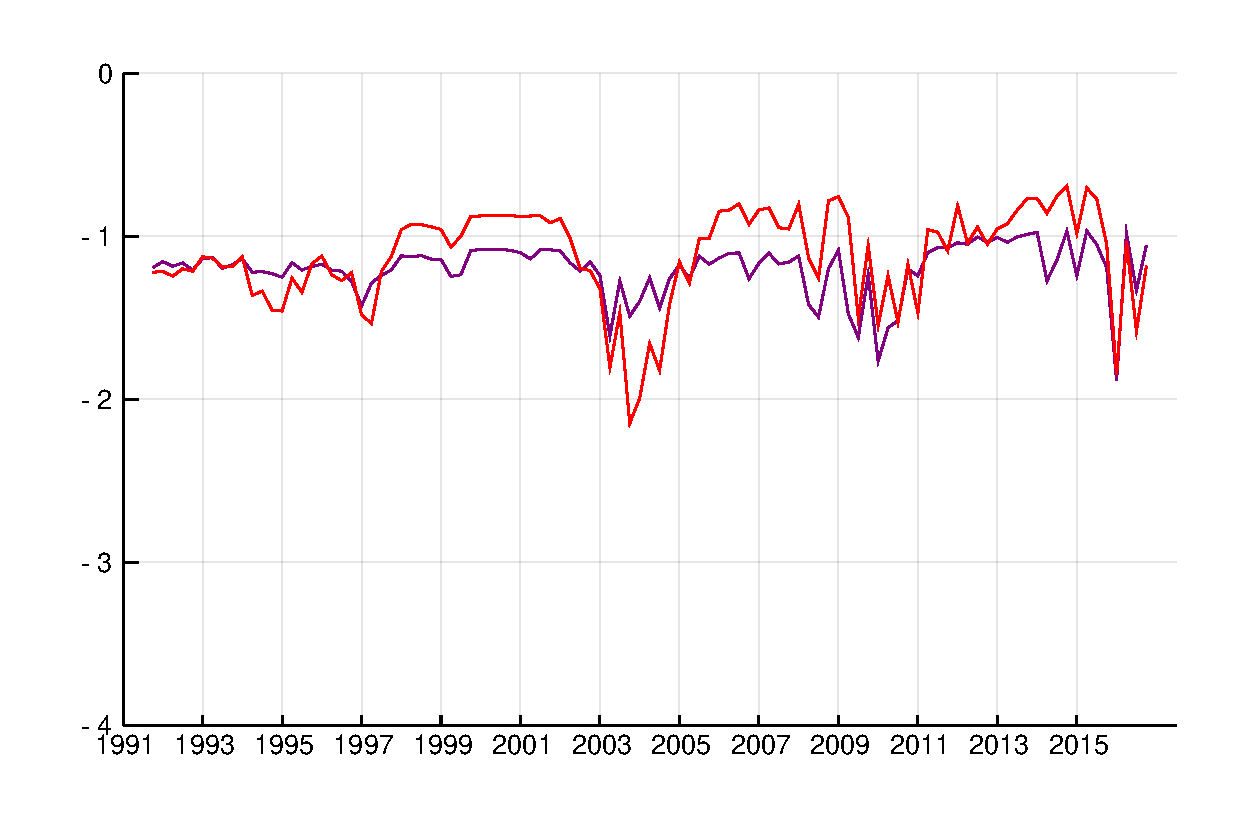
\includegraphics[height=1.5in,width=.45\textwidth,angle=0,clip, trim=.1cm .1cm .1cm .1cm]{\plotroot/forecasting/predictive_densities/standard_prior/pred_densities_gdp/SWvm904/grouped_mean_pred_dens_both_hor=8_T0=1991-12-31_T=2016-12-31.pdf} \\[-.5ex]
            \multicolumn{2}{c}{Conditioning on Nowcasts} \\[-.5ex]
            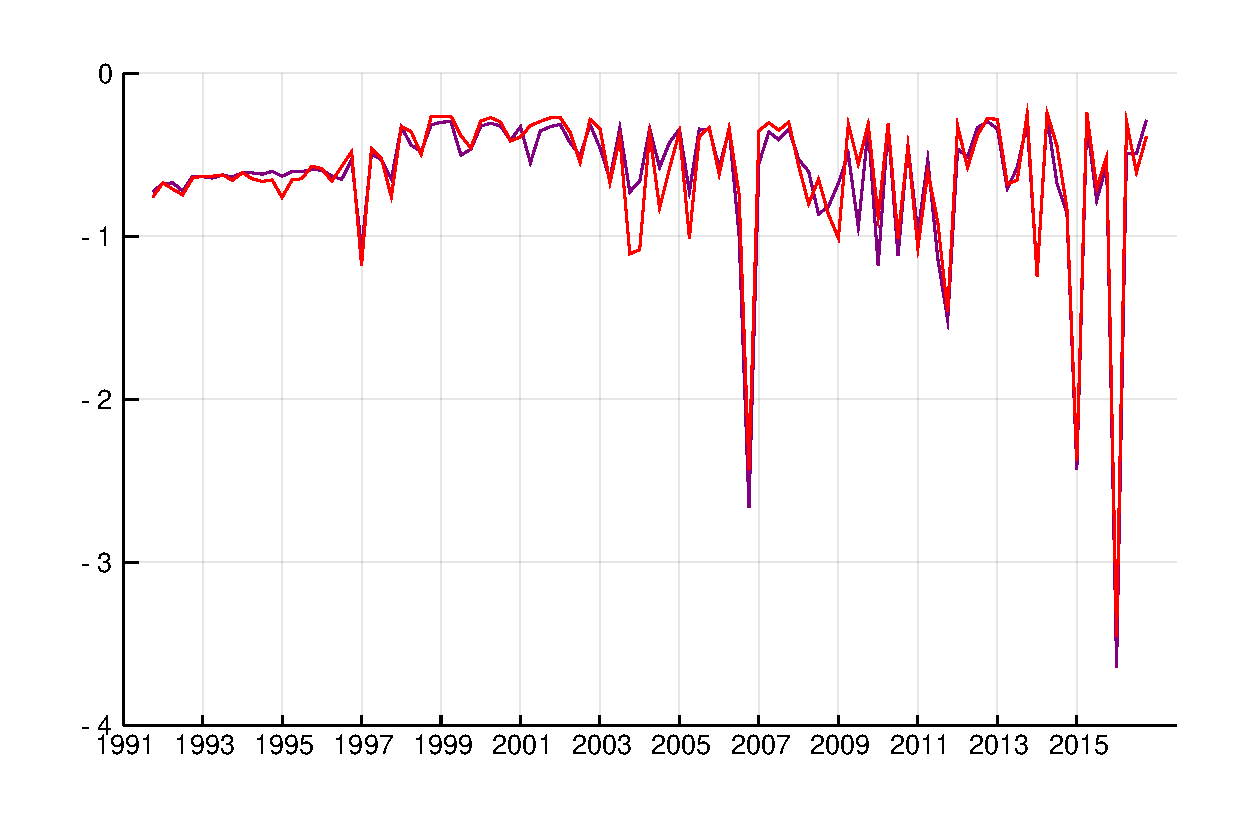
\includegraphics[height=1.5in,width=.45\textwidth,angle=0,clip, trim=.1cm .1cm .1cm .1cm]{\plotroot/forecasting/predictive_densities/standard_prior/pred_densities_gdp/SWvm904/grouped_mean_pred_dens_nowcast_hor=2_T0=1991-12-31_T=2016-12-31.pdf} &
            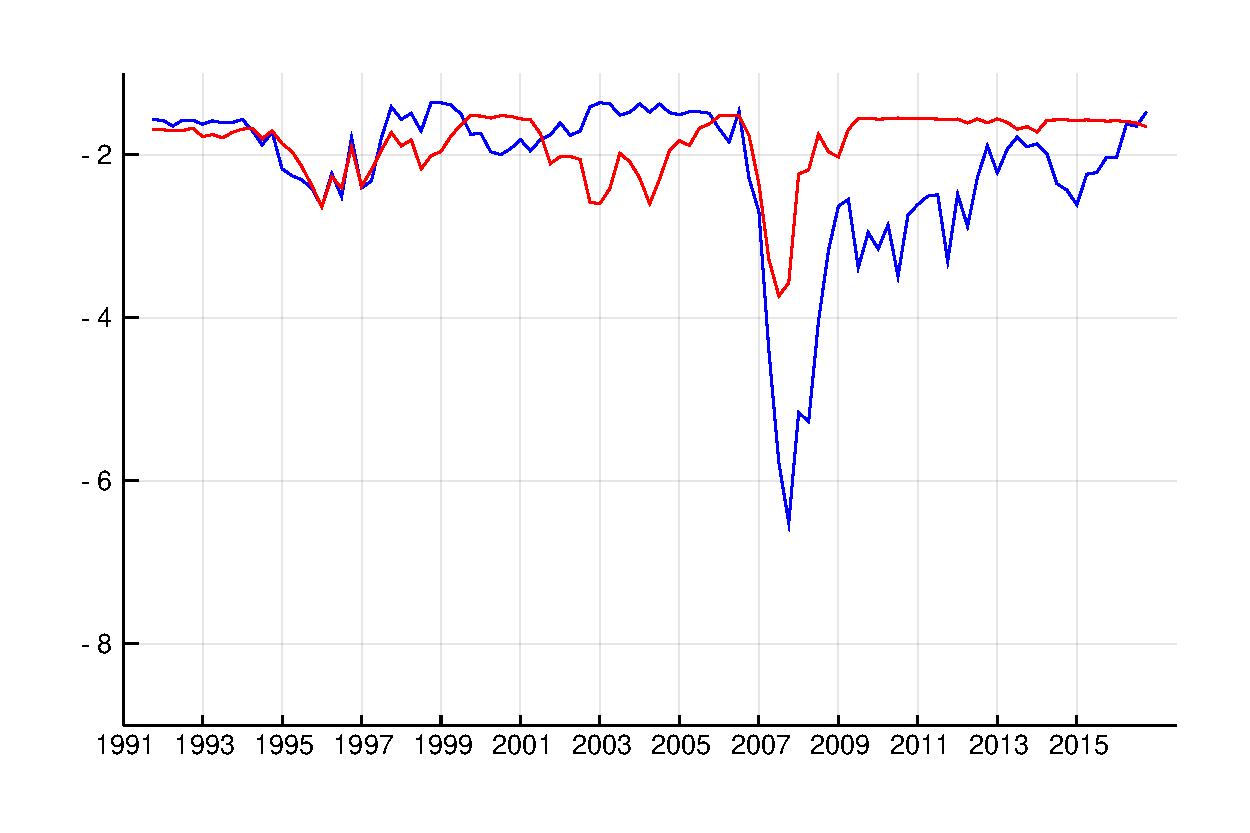
\includegraphics[height=1.5in,width=.45\textwidth,angle=0,clip, trim=.1cm .1cm .1cm .1cm]{\plotroot/forecasting/predictive_densities/standard_prior/pred_densities_gdp/SWvm904/grouped_mean_pred_dens_nowcast_hor=8_T0=1991-12-31_T=2016-12-31.pdf} \\[-.5ex]
            \multicolumn{2}{c}{Conditioning on FFR Expectations} \\[-.5ex]
            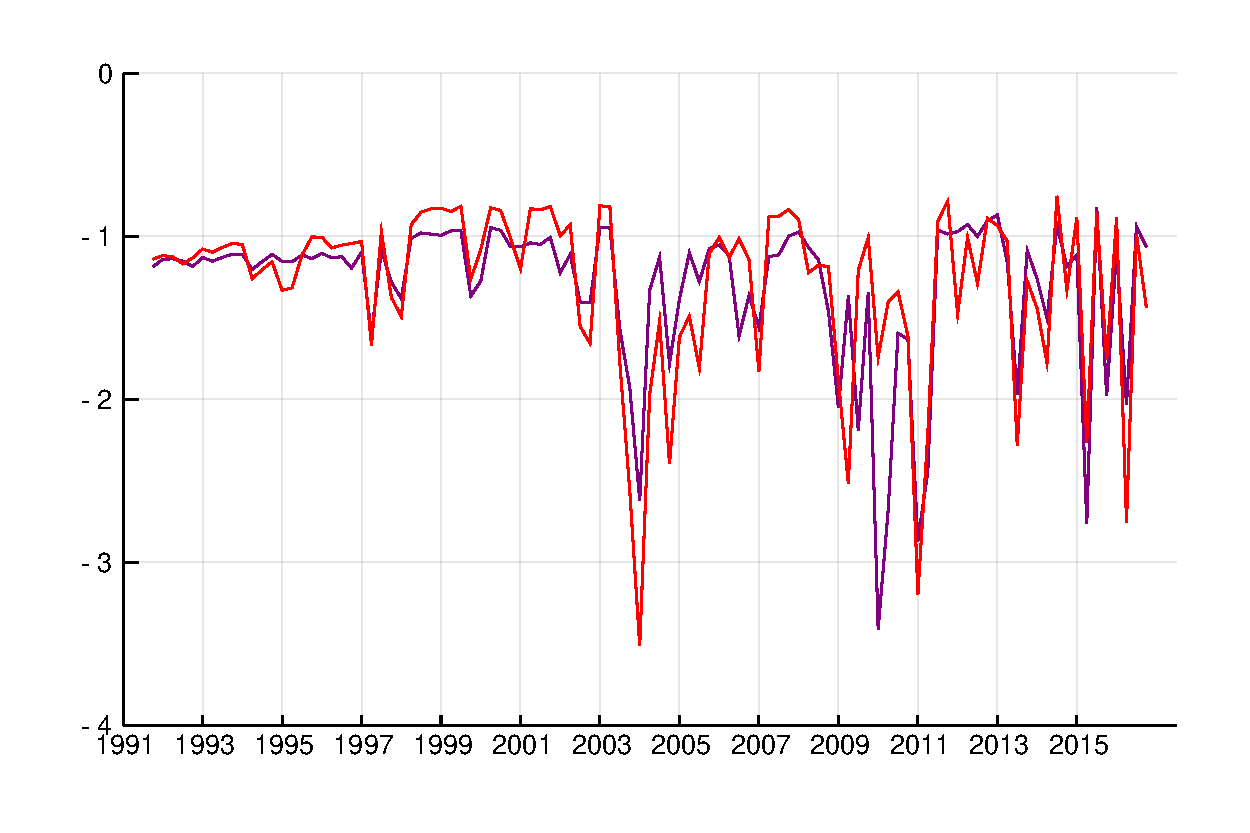
\includegraphics[height=1.5in,width=.45\textwidth,angle=0,clip, trim=.1cm .1cm .1cm .1cm]{\plotroot/forecasting/predictive_densities/standard_prior/pred_densities_gdp/SWvm904/grouped_mean_pred_dens_bluechip_hor=2_T0=1991-12-31_T=2016-12-31.pdf} &
            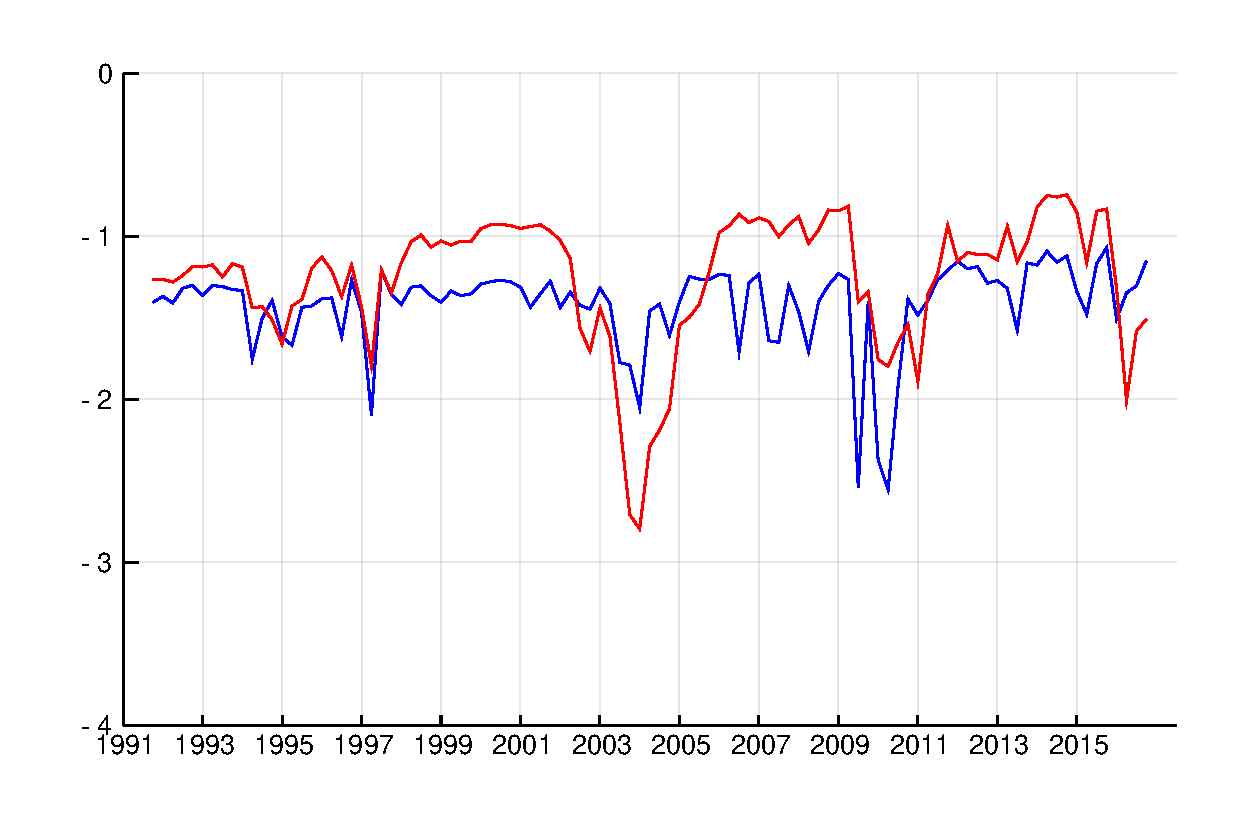
\includegraphics[height=1.5in,width=.45\textwidth,angle=0,clip, trim=.1cm .1cm .1cm .1cm]{\plotroot/forecasting/predictive_densities/standard_prior/pred_densities_gdp/SWvm904/grouped_mean_pred_dens_bluechip_hor=8_T0=1991-12-31_T=2016-12-31.pdf} \\[-.5ex]
            \multicolumn{2}{c}{Conditioning on Neither} \\[-.5ex]
            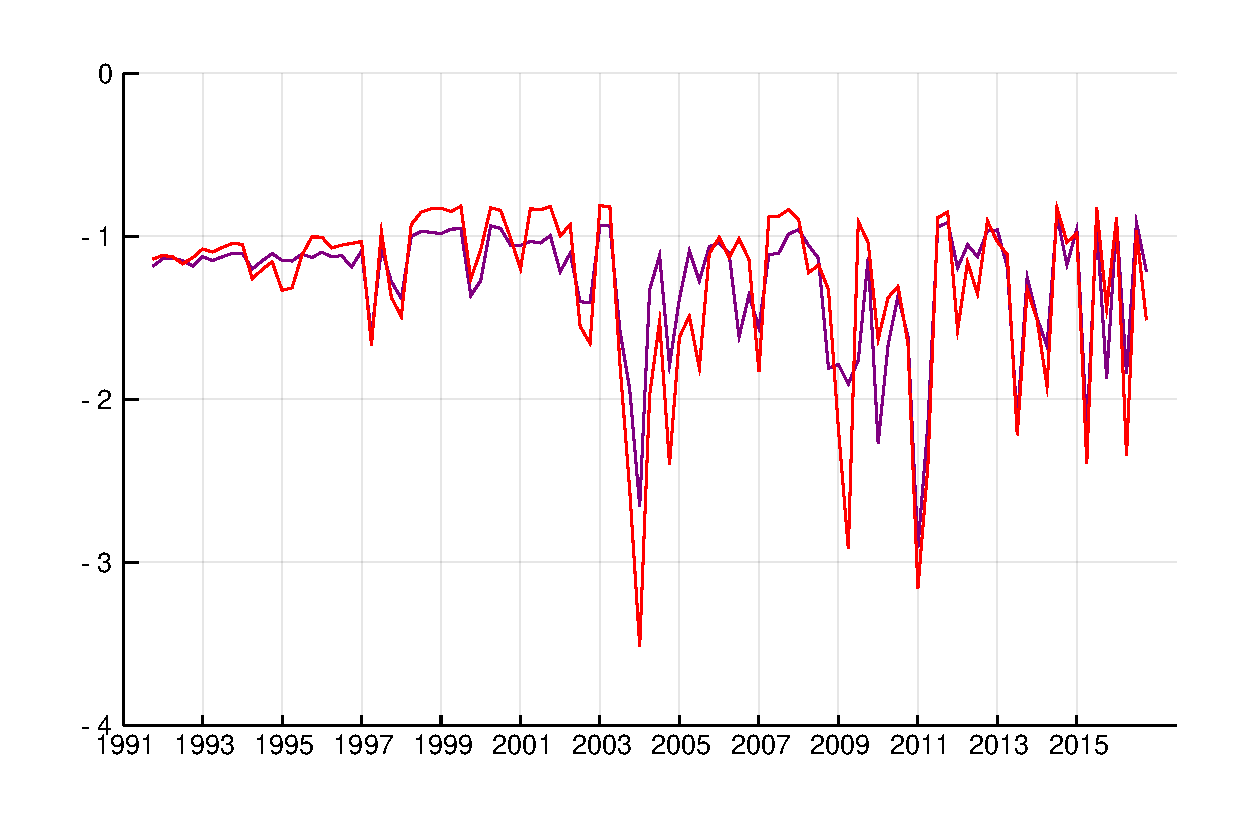
\includegraphics[height=1.5in,width=.45\textwidth,angle=0,clip, trim=.1cm .1cm .1cm .1cm]{\plotroot/forecasting/predictive_densities/standard_prior/pred_densities_gdp/SWvm904/grouped_mean_pred_dens_neither_hor=2_T0=1991-12-31_T=2016-12-31.pdf} &
            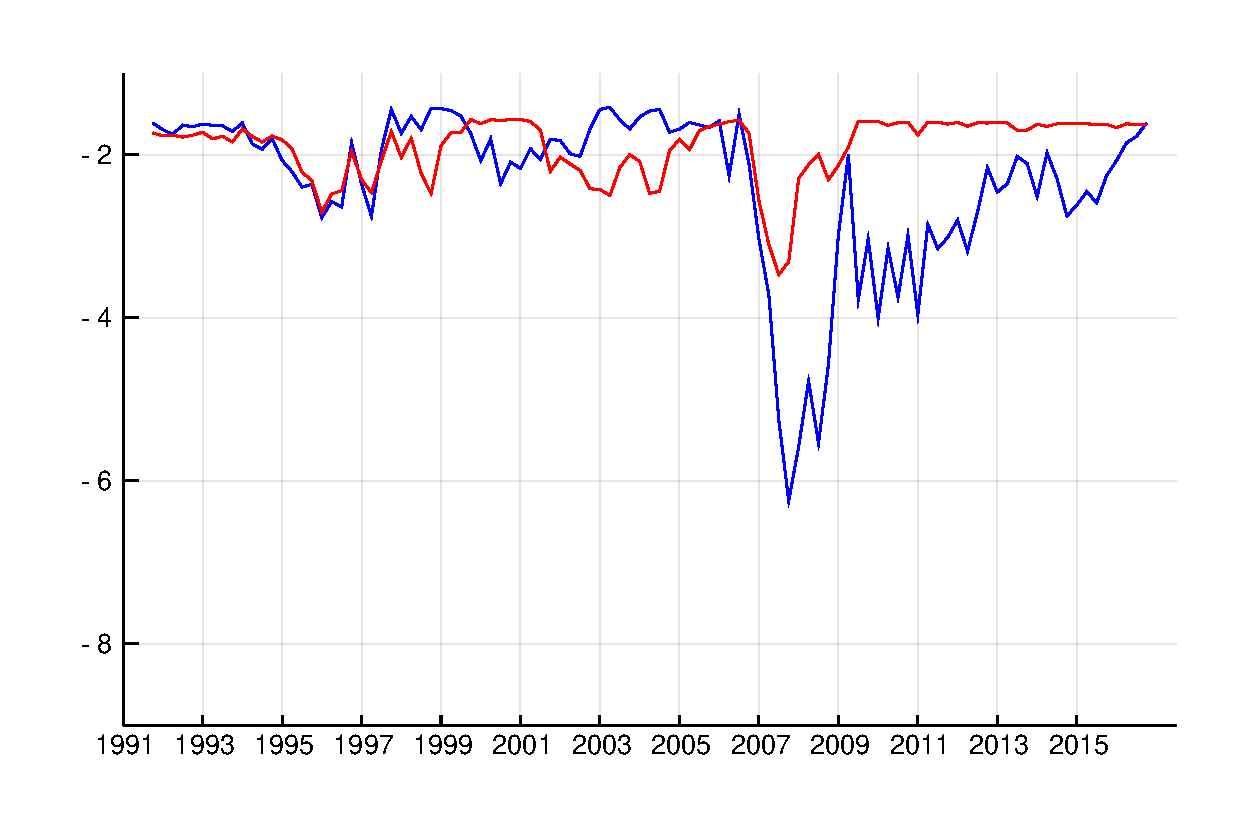
\includegraphics[height=1.5in,width=.45\textwidth,angle=0,clip, trim=.1cm .1cm .1cm .1cm]{\plotroot/forecasting/predictive_densities/standard_prior/pred_densities_gdp/SWvm904/grouped_mean_pred_dens_neither_hor=8_T0=1991-12-31_T=2016-12-31.pdf} \\[-.5ex]
        \end{tabular}
    \end{center}
    \begin{minipage}{\textwidth}
    \vspace{-.5cm}
    \scriptsize
    \setlength{\baselineskip}{2mm}
    \emph{Note}: These panels compare $\log p(\bar{y}_{t+h, h} | \mathcal{I}^m_{t},\mathcal{M}_{m})$ from the SW DSGE model (blue) with the SWFF DSGE model (red) averaged over two, four, six, and eight quarter horizons for output growth. Forecast origins from January 1992 to January 2017 only are included in these calculations. The x-axis shows the quarter in which the forecasts were generated (time $T+1$ in the parlance of section \ref{subsec:realtimedata}).
    \end{minipage}
\end{figure}



 \begin{figure}[H]
    \caption{Average Log Predictive Density Scores for SW vs SWFF: Post-Recession Sample}
    \label{fig:avgpreddens_sw_vs_swff_post_recession}
      \vspace*{-0.75cm}
  \begin{center}
        \begin{tabular}{@{\hspace*{-.4cm}}ccc}
            GDP & GDP Deflator & GDP and GDP Deflator \\[-.5ex]
            \multicolumn{3}{c}{Conditioning on FFR Expectations} \\[-.5ex]
            \includegraphics[height=1.5in,width=.32\textwidth,angle=0,clip, trim=.1cm .1cm .1cm .1cm]{\plotroot/forecasting/predictive_densities/standard_prior/pred_densities_gdp/SWvm904/time_averaged_sw_vs_swff_bluechip_T0=2011-03-31_T=2016-03-31.pdf} &
            \includegraphics[height=1.5in,width=.32\textwidth,angle=0,clip, trim=.1cm .1cm .1cm .1cm]{\plotroot/forecasting/predictive_densities/standard_prior/pred_densities_def/SWvm904/time_averaged_sw_vs_swff_bluechip_T0=2011-03-31_T=2016-03-31.pdf} &
            \includegraphics[height=1.5in,width=.32\textwidth,angle=0,clip, trim=.1cm .1cm .1cm .1cm]{\plotroot/forecasting/predictive_densities/standard_prior/pred_densities_both/SWvm904/time_averaged_sw_vs_swff_bluechip_T0=2011-03-31_T=2016-03-31.pdf} \\[-.5ex]
            \multicolumn{3}{c}{Conditioning on Neither} \\[-.5ex]
            \includegraphics[height=1.5in,width=.32\textwidth,angle=0,clip, trim=.1cm .1cm .1cm .1cm]{\plotroot/forecasting/predictive_densities/standard_prior/pred_densities_gdp/SWvm904/time_averaged_sw_vs_swff_neither_T0=2011-03-31_T=2016-03-31.pdf} &
            \includegraphics[height=1.5in,width=.32\textwidth,angle=0,clip, trim=.1cm .1cm .1cm .1cm]{\plotroot/forecasting/predictive_densities/standard_prior/pred_densities_def/SWvm904/time_averaged_sw_vs_swff_neither_T0=2011-03-31_T=2016-03-31.pdf} &
            \includegraphics[height=1.5in,width=.32\textwidth,angle=0,clip, trim=.1cm .1cm .1cm .1cm]{\plotroot/forecasting/predictive_densities/standard_prior/pred_densities_both/SWvm904/time_averaged_sw_vs_swff_neither_T0=2011-03-31_T=2016-03-31.pdf} \\[-.5ex]
        \end{tabular}
    \end{center}
    \begin{minipage}{\textwidth}
        \vspace{-.5cm}
        \scriptsize
        \setlength{\baselineskip}{2mm}
        \emph{Note}: These panels compare the log predictive densities from the SW DSGE model (blue diamonds) and with the SWFF DSGE model (red diamonds) averaged over two, four, six, and eight quarter horizons for output growth and inflation individually, and for both together. Forecast origins from April 2011 to April 2016 only are included in these calculations.
    \end{minipage}
 \end{figure}
\clearpage
\subsection{Log Predictive Density Scores with Diffuse Priors}
\label{subsec:forecasting_diffuseprior}
\begin{figure}[H]
    \caption{Comparison of  Predictive Densities  under Standard and Diffuse Priors}
    \label{fig:avgpreddens_standard_vs_diffuse_whole_sample}
    \begin{tabular}{@{\hspace*{-.4cm}}ccc}
        GDP & GDP Deflator & GDP and GDP Deflator \\[-.5ex]
        \multicolumn{3}{c}{SW}\\[-.5ex]
        \includegraphics[height=1.5in,width=.32\textwidth,angle=0,clip, trim=.1cm .1cm .1cm .1cm]{\plotroot/forecasting/predictive_densities/prior_comparison/pred_densities_gdp/smets_wouters/time_averaged_sw_prior_comparison_both_T0=1991-12-31_T=2016-12-31.pdf} &
        \includegraphics[height=1.5in,width=.32\textwidth,angle=0,clip, trim=.1cm .1cm .1cm .1cm]{\plotroot/forecasting/predictive_densities/prior_comparison/pred_densities_def/smets_wouters/time_averaged_sw_prior_comparison_both_T0=1991-12-31_T=2016-12-31.pdf} &
        \includegraphics[height=1.5in,width=.32\textwidth,angle=0,clip, trim=.1cm .1cm .1cm .1cm]{\plotroot/forecasting/predictive_densities/prior_comparison/pred_densities_both/smets_wouters/time_averaged_sw_prior_comparison_both_T0=1991-12-31_T=2016-12-31.pdf} \\[-.5ex]
        \multicolumn{3}{c}{SW$\pi$}\\[-.5ex]
        \includegraphics[height=1.5in,width=.32\textwidth,angle=0,clip, trim=.1cm .1cm .1cm .1cm]{\plotroot/forecasting/predictive_densities/prior_comparison/pred_densities_gdp/m805/time_averaged_swpi_prior_comparison_both_T0=1991-12-31_T=2016-12-31.pdf} &
        \includegraphics[height=1.5in,width=.32\textwidth,angle=0,clip, trim=.1cm .1cm .1cm .1cm]{\plotroot/forecasting/predictive_densities/prior_comparison/pred_densities_def/m805/time_averaged_swpi_prior_comparison_both_T0=1991-12-31_T=2016-12-31.pdf} &
        \includegraphics[height=1.5in,width=.32\textwidth,angle=0,clip, trim=.1cm .1cm .1cm .1cm]{\plotroot/forecasting/predictive_densities/prior_comparison/pred_densities_both/m805/time_averaged_swpi_prior_comparison_both_T0=1991-12-31_T=2016-12-31.pdf} \\[-.5ex]
        \multicolumn{3}{c}{SWFF Model}\\[-.5ex]
        \includegraphics[height=1.5in,width=.32\textwidth,angle=0,clip, trim=.1cm .1cm .1cm .1cm]{\plotroot/forecasting/predictive_densities/prior_comparison/pred_densities_gdp/m904/time_averaged_swff_prior_comparison_both_T0=1991-12-31_T=2016-12-31.pdf} &
        \includegraphics[height=1.5in,width=.32\textwidth,angle=0,clip, trim=.1cm .1cm .1cm .1cm]{\plotroot/forecasting/predictive_densities/prior_comparison/pred_densities_def/m904/time_averaged_swff_prior_comparison_both_T0=1991-12-31_T=2016-12-31.pdf} &
        \includegraphics[height=1.5in,width=.32\textwidth,angle=0,clip, trim=.1cm .1cm .1cm .1cm]{\plotroot/forecasting/predictive_densities/prior_comparison/pred_densities_both/m904/time_averaged_swff_prior_comparison_both_T0=1991-12-31_T=2016-12-31.pdf} \\[-.5ex]
    \end{tabular}
    \begin{minipage}{\textwidth}
        \scriptsize
        \setlength{\baselineskip}{2mm}
        \emph{Note}: These panels compare the predictive densities estimated with the standard   (solid line) and the diffuse  (dashed line) prior for the SW (blue, top row), SW$\pi$ (purple, middle row), and SWFF (red, bottom row) DSGE models. The predictive densities are averaged over two, four, six, and eight quarter horizons for output growth and inflation individually, and for both together. Forecast origins fro\
m January 1992 to January 2017 only are included in these calculations. The forecasts associated with these predictive densities are generated conditioning on nowcasts and FFR expectations.
    \end{minipage}
\end{figure}

This section contains additional details relating to the results reported in the main paper. In Section~\ref{appsubsec:mh35} we show summary tables for the performance of the SMC algorith on the AS and SW models for $N_\text{MH}=3$ and $N_\text{MH}=5$. In Section~\ref{appsubsec:predictive_densities_over_time} we show the evolution of log predictive scores over time. 

\subsection{Summary Statistics for $N_\text{MH}=3$ and $N_\text{MH}=5$}

\label{appsubsec:mh35}
\begin{table}[H]
	\caption{AS Model: 3 MH Steps Per Mutation}
	\label{appsubsec:as.smcsummary}
	\begin{center}
		\begin{tabular} {lrrrrrr} 
 \hline \hline 
&Fixed&$\alpha = $0.90&$\alpha = $0.95&$\alpha = $0.97&$\alpha = $0.98\\ 
 \hline 
Mean log(MDD)&-1032.00&-1032.44&-1032.01&-1031.84&-1031.76\\ 
StdD log(MDD)&0.28&0.46&0.23&0.15&0.11\\ 
Schedule Length&200.00&106.52&197.56&300.72&413.46\\ 
Resamples&12.98&14.75&13.75&12.73&11.04\\ 
Runtime [Min]&2.25&1.35&2.31&3.22&4.34\\ 
\hline 
\end{tabular}
	\end{center}
	%\hspace*{-1cm}
	{\footnotesize {\em Notes:} Results are based on $N_{run} = 400$ runs of the SMC algorithm. We report averages across runs for the runtime, schedule length, and number of resampling steps.}\setlength{\baselineskip}{4mm}
\end{table}

\begin{table}[H]
	\caption{AS Model: 5 MH Steps Per Mutation}
	\label{appsubsec:as.smcsummary}
	\begin{center}
		\begin{tabular} {lrrrrrr} 
 \hline \hline 
&Fixed&$\alpha = $0.90&$\alpha = $0.95&$\alpha = $0.97&$\alpha = $0.98\\ 
 \hline 
Mean log(MDD)&-1032.03&-1032.44&-1032.07&-1031.94&-1031.89\\ 
StdD log(MDD)&0.24&0.41&0.21&0.14&0.11\\ 
Schedule Length&200.00&104.36&190.29&286.06&389.48\\ 
Resamples&12.06&14.11&13.00&12.00&10.93\\ 
Runtime [Min]&3.08&1.73&2.90&3.98&5.34\\ 
\hline 
\end{tabular}
	\end{center}
	%\hspace*{-1cm}
	{\footnotesize {\em Notes:} Results are based on $N_{run} = 400$ runs of the SMC algorithm. We report averages across runs for the runtime, schedule length, and number of resampling steps.}\setlength{\baselineskip}{4mm}
\end{table}

\clearpage

\begin{table}[H]
	\caption{SW Model: 3 MH Steps Per Mutation}
	\label{appsubsec:sw.smcsummary}
	\begin{center}
		\begin{tabular} {lrrrrrr} 
 \hline \hline 
&Fixed&$\alpha = $0.90&$\alpha = $0.95&$\alpha = $0.97&$\alpha = $0.98\\ 
 \hline 
Mean log(MDD)&-1176.76&-1179.65&-1177.76&-1176.99&-1176.65\\ 
StdD log(MDD)&0.75&1.35&0.87&0.84&0.65\\ 
Schedule Length&500.00&191.58&355.68&547.25&760.71\\ 
Resamples&24.59&26.95&25.03&23.33&21.15\\ 
Runtime [Min]&207.66&73.59&137.32&211.64&293.92\\ 
\hline 
\end{tabular}
	\end{center}
	%\hspace*{-1cm}
	{\footnotesize {\em Notes:} Results are based on $N_{run} = 200$ runs of the SMC algorithm. We report averages across runs for the runtime, schedule length, and number of resampling steps.}\setlength{\baselineskip}{4mm}
\end{table}



\begin{table}[H]
	\caption{SW Model: 5 MH Steps Per Mutation}
	\label{appsubsec:sw.smcsummary}
	\begin{center}
		\begin{tabular} {lrrrrrr} 
 \hline \hline 
&Fixed&$\alpha = $0.90&$\alpha = $0.95&$\alpha = $0.97&$\alpha = $0.98\\ 
 \hline 
Mean log(MDD)&-1176.70&-1179.04&-1177.52&-1176.89&-1176.62\\ 
StdD log(MDD)&0.50&1.27&0.80&0.73&0.51\\ 
Schedule Length&500.00&188.14&346.19&525.90&721.36\\ 
Resamples&23.27&26.23&24.20&22.33&20.04\\ 
Runtime [Min]&324.15&110.10&202.83&311.21&424.92\\ 
\hline 
\end{tabular}
	\end{center}
	%\hspace*{-1cm}
	{\footnotesize {\em Notes:} Results are based on $N_{run} = 200$ runs of the SMC algorithm. We report averages across runs for the runtime, schedule length, and number of resampling steps.}\setlength{\baselineskip}{4mm}
\end{table}

\clearpage

\subsection{Log Predictive Scores Over Time}
\label{appsubsec:predictive_densities_over_time}
% Whole Sample

\begin{figure}[h!]
  \caption{GDP Log Predictive Scores Over Time for SW vs SWFF}
  \vspace*{-0.75cm}
  \begin{center}
    \begin{tabular}{cc}
      Horizon = 2 & Horizon = 4 \\[-.5ex]	
      \includegraphics[width=.48\textwidth,angle=0,clip, trim=.1cm .1cm .1cm .1cm]{\plotroot/forecasting/predictive_densities/standard_prior/pred_densities_gdp/SWvm904/grouped_mean_pred_dens_both_hor=2_T0=1991-12-31_T=2016-12-31.pdf} &
      \includegraphics[width=.48\textwidth,angle=0,clip, trim=.1cm .1cm .1cm .1cm]{\plotroot/forecasting/predictive_densities/standard_prior/pred_densities_gdp/SWvm904/grouped_mean_pred_dens_both_hor=4_T0=1991-12-31_T=2016-12-31.pdf} \\[-.5ex]
      Horizon = 6 & Horizon = 8 \\[-.5ex]	
\includegraphics[width=.48\textwidth,angle=0,clip, trim=.1cm .1cm .1cm .1cm]{\plotroot/forecasting/predictive_densities/standard_prior/pred_densities_gdp/SWvm904/grouped_mean_pred_dens_both_hor=6_T0=1991-12-31_T=2016-12-31.pdf} &
      \includegraphics[width=.48\textwidth,angle=0,clip, trim=.1cm .1cm .1cm .1cm]{\plotroot/forecasting/predictive_densities/standard_prior/pred_densities_gdp/SWvm904/grouped_mean_pred_dens_both_hor=8_T0=1991-12-31_T=2016-12-31.pdf} 
      \end{tabular}
  \end{center}
  \begin{minipage}{\textwidth}
    \vspace{-.5cm}
    \scriptsize
    \setlength{\baselineskip}{2mm}
    \emph{Note}: The four panels show the predictive density comparisons across time for the SW (blue line) and SWFF (red line) DSGE models averaged over 2, 4, 6, and 8 quarter horizons for output growth. Forecast origins from January 1992 to January 2017 only are included in these calculations. The x-axis shows the quarter in which the forecasts were generated (time $T+1$ in the parlance of section \ref{subsec:realtimedata}).
  \end{minipage}
\end{figure}

%\pagebreak
\begin{figure}[h!]
	\caption{GDP Deflator Log Predictive Scores Over Time for SW vs SWFF}
	\vspace*{-0.75cm}
	\begin{center}
		\begin{tabular}{cc}
			Horizon = 2 & Horizon = 4 \\[-.5ex]	
			\includegraphics[width=.48\textwidth,angle=0,clip, trim=.1cm .1cm .1cm .1cm]{\plotroot/forecasting/predictive_densities/standard_prior/pred_densities_def/SWvm904/grouped_mean_pred_dens_both_hor=2_T0=1991-12-31_T=2016-12-31.pdf} &
			\includegraphics[width=.48\textwidth,angle=0,clip, trim=.1cm .1cm .1cm .1cm]{\plotroot/forecasting/predictive_densities/standard_prior/pred_densities_def/SWvm904/grouped_mean_pred_dens_both_hor=4_T0=1991-12-31_T=2016-12-31.pdf} \\[-.5ex]
			Horizon = 6 & Horizon = 8 \\[-.5ex]	
			\includegraphics[width=.48\textwidth,angle=0,clip, trim=.1cm .1cm .1cm .1cm]{\plotroot/forecasting/predictive_densities/standard_prior/pred_densities_def/SWvm904/grouped_mean_pred_dens_both_hor=6_T0=1991-12-31_T=2016-12-31.pdf} &
			\includegraphics[width=.48\textwidth,angle=0,clip, trim=.1cm .1cm .1cm .1cm]{\plotroot/forecasting/predictive_densities/standard_prior/pred_densities_def/SWvm904/grouped_mean_pred_dens_both_hor=8_T0=1991-12-31_T=2016-12-31.pdf} 
      \end{tabular}
  \end{center}
  \begin{minipage}{\textwidth}
    \vspace{-.5cm}
    \scriptsize
    \setlength{\baselineskip}{2mm}
    \emph{Note}: The four panels show the predictive density comparisons across time for the SW (blue line) and SWFF (red line) DSGE models averaged over 2, 4, 6, and 8 quarter horizons for inflation. Forecast origins from January 1992 to January 2017 only are included in these calculations. The x-axis shows the quarter in which the forecasts were generated (time $T+1$ in the parlance of section \ref{subsec:realtimedata}).
  \end{minipage}
\end{figure}

%\pagebreak
\begin{figure}[h!]
	\caption{GDP Deflator Log Predictive Scores Over Time for SW vs SWFF}
	\vspace*{-0.75cm}
	\begin{center}
		\begin{tabular}{cc}
			Horizon = 2 & Horizon = 4 \\[-.5ex]	
			\includegraphics[width=.48\textwidth,angle=0,clip, trim=.1cm .1cm .1cm .1cm]{\plotroot/forecasting/predictive_densities/standard_prior/pred_densities_both/SWvm904/grouped_mean_pred_dens_both_hor=2_T0=1991-12-31_T=2016-12-31.pdf} &
			\includegraphics[width=.48\textwidth,angle=0,clip, trim=.1cm .1cm .1cm .1cm]{\plotroot/forecasting/predictive_densities/standard_prior/pred_densities_both/SWvm904/grouped_mean_pred_dens_both_hor=4_T0=1991-12-31_T=2016-12-31.pdf} \\[-.5ex]
			Horizon = 6 & Horizon = 8 \\[-.5ex]	
			\includegraphics[width=.48\textwidth,angle=0,clip, trim=.1cm .1cm .1cm .1cm]{\plotroot/forecasting/predictive_densities/standard_prior/pred_densities_both/SWvm904/grouped_mean_pred_dens_both_hor=6_T0=1991-12-31_T=2016-12-31.pdf} &
			\includegraphics[width=.48\textwidth,angle=0,clip, trim=.1cm .1cm .1cm .1cm]{\plotroot/forecasting/predictive_densities/standard_prior/pred_densities_def/SWvm904/grouped_mean_pred_dens_both_hor=8_T0=1991-12-31_T=2016-12-31.pdf} 
      \end{tabular}
  \end{center}
  \begin{minipage}{\textwidth}
    \vspace{-.5cm}
    \scriptsize
    \setlength{\baselineskip}{2mm}
    \emph{Note}: The four panels show the predictive density comparisons across time for the SW (blue line) and SWFF (red line) DSGE models averaged over 2, 4, 6, and 8 quarter horizons for output growth and inflation. Forecast origins from January 1992 to January 2017 only are included in these calculations. The x-axis shows the quarter in which the forecasts were generated (time $T+1$ in the parlance of section \ref{subsec:realtimedata}).
  \end{minipage}
\end{figure}


\end{document}
